\smalltitle{سوال 2}\\
% r = np.array([ 1,  2, -1,  0])
% a = np.array([[1,1,1,1],r,r**2,r**3]).T
% np.matrix((a.T)@a).I @ a.T @ np.array([[1],[0],[2],[-1]])
\smalltitle{الف}
\begin{gather*}
    \begin{bmatrix}
        1 & 1\\
        1 & 2\\
        1 & -1\\
        1 & 0
    \end{bmatrix}
    \begin{bmatrix}
        a\\b
    \end{bmatrix}
    =
    \begin{bmatrix}
        1\\0\\2\\-1
    \end{bmatrix}
    \\\implies
    \hat{x} = (A^TA)^{-1} A^T b
    = \begin{bmatrix}
        4 & 2\\
        2 & 6
    \end{bmatrix}^{-1}
    \begin{bmatrix}
        1 & 1 & 1 & 1\\
        1 & 2 & -1 & 0
    \end{bmatrix}
    \begin{bmatrix}
        1\\0\\2\\-1
    \end{bmatrix}
    \\=
    \begin{bmatrix}
        0.3 & -0.1\\
        -0.1 & 0.2
    \end{bmatrix}
    \begin{bmatrix}
        1 & 1 & 1 & 1\\
        1 & 2 & -1 & 0
    \end{bmatrix}
    \begin{bmatrix}
        1\\0\\2\\-1
    \end{bmatrix}
    = \begin{bmatrix}
        0.7 \\ -0.4
    \end{bmatrix}
    \\
    error = \frac{\begin{vmatrix}
        1 - (0.7 - 0.4 \times 1)\\
        0 - (0.7 - 0.4 \times 2)\\
        2 - (0.7 - 0.4 \times -1)\\
        -1 - (0.7 - 0.4 \times 0)
    \end{vmatrix}}{4}
    = 
    \frac{\begin{vmatrix}
        0.7\\
        0.1\\
        0.9\\
        -1.7
    \end{vmatrix}}{4}
    = \frac{4.2}{4}
\end{gather*}
\smalltitle{ب}
\begin{gather*}
    \begin{bmatrix}
        1 & 1 & 1\\
        1 & 2 & 4\\
        1 & -1 & 1\\
        1 & 0 & 0
    \end{bmatrix}
    \begin{bmatrix}
        a\\b\\c
    \end{bmatrix}
    =
    \begin{bmatrix}
        1\\0\\2\\-1
    \end{bmatrix}
    \\\implies
    \begin{bmatrix}
        a\\b\\c
    \end{bmatrix}
    =
    \begin{bmatrix}
        0.2\\-0.9\\0.5
    \end{bmatrix}\\
    error = \frac{\begin{vmatrix}
        1 - (0.2 - 0.9 \times 1 +  0.5 \times (1 )^2)\\
        0 - (0.2 - 0.9 \times 2 +  0.5 \times (2 )^2)\\
        2 - (0.2 - 0.9 \times -1 + 0.5 \times (-1)^2)\\
        -1 - (0.2 - 0.9 \times 0 + 0.5 \times ( 0)^2)
    \end{vmatrix}}{4}
    = 
    \frac{\begin{vmatrix}
        1.2\\
        -0.4\\
        0.4\\
        -1.2
    \end{vmatrix}}{4}
    = \frac{3.2}{4}
\end{gather*}
\smalltitle{ج}
% (1,1),(2,0),(-1,2),(0,-1)
% f\left(x\right)=0.7-0.4x
% g\left(x\right)=0.2-0.9x+0.5x^{2}
\begin{figure}[H]
    \centerline{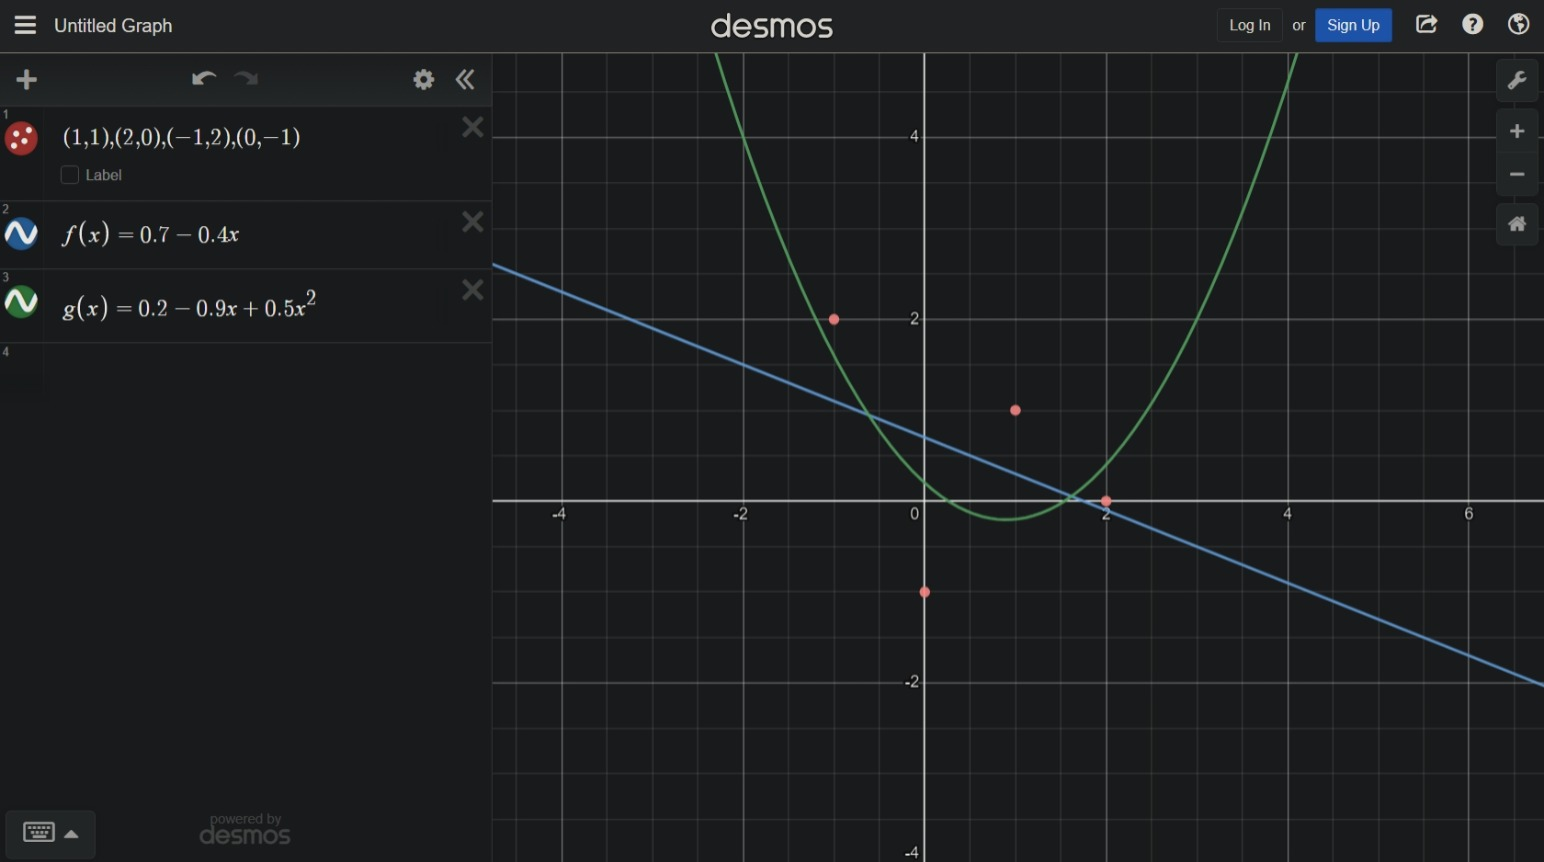
\includegraphics[scale=0.275]{pics/2-3.jpeg}}
\end{figure}
\noindent
به نظر من هیچ کدام از این تخمین‌ها مناسب نیستند. چرا که در کل نقاط داده شده پراکندگی زیادی دارند و نمی‌توان
آنها را به توابع درجه پایین نسبت داد. البته دقت کنید که زمانی که درجه‌ی معادله را به پنج برسانیم
خط از نقاط رد می‌شود.





